
\documentclass{beamer}
\usecolortheme{dove}
\setbeamertemplate{navigation symbols}{}
\usepackage{amsmath,amssymb,amsfonts,amsthm, multicol, subfigure, color}
\setbeamertemplate{footline}[text line]{\parbox{\linewidth}{\vspace*{-8pt}\bgray{Resampling for Inference} \insertsectionnavigationhorizontal{.75\paperwidth}{}{\hfill\hfill}}}
\usepackage{bm}
\usepackage{graphicx}
\usepackage{tabularx}
\usepackage{booktabs}
\usepackage{hyperref}
\usepackage{pdfpages}
\usepackage{xcolor}
\definecolor{seagreen}{RGB}{46, 139, 87}
\def\independenT#1#2{\mathrel{\rlap{$#1#2$}\mkern2mu{#1#2}}}
\newcommand\indep{\protect\mathpalette{\protect\independenT}{\perp}}
\def\log{\text{log}}
\newcommand\logit{\text{logit}}
\newcommand\iid{\stackrel{\text{iid}}{\sim}}
\newcommand\E{\text{E}}
\newcommand\V{\text{V}}
\renewcommand\P{\text{P}}
\newcommand{\Cov}{\text{Cov}}
\newcommand{\Cor}{\text{Cor}}
\newcommand\doop{\texttt{do}}
\usepackage{stackrel}
\usepackage{tikz}
\usetikzlibrary{arrows,shapes.arrows,positioning,shapes,patterns,calc}
\newcommand\slideref[1]{\vskip .1cm \tiny \textcolor{gray}{{#1}}}
\newcommand\red[1]{\color{red}#1}
\newcommand\blue[1]{\color{blue}#1}
\newcommand\gray[1]{\color{gray}#1}
\newcommand\seagreen[1]{\color{seagreen}#1}
\newcommand\purple[1]{\color{purple}#1}
\newcommand\orange[1]{\color{orange}#1}
\newcommand\black[1]{\color{black}#1}
\newcommand\white[1]{\color{white}#1}
\newcommand\teal[1]{\color{teal}#1}
\newcommand\magenta[1]{\color{magenta}#1}
\newcommand\Fuchsia[1]{\color{Fuchsia}#1}
\newcommand\BlueGreen[1]{\color{BlueGreen}#1}
\newcommand\bblue[1]{\textcolor{blue}{\textbf{#1}}}
\newcommand\bred[1]{\textcolor{red}{\textbf{#1}}}
\newcommand\bgray[1]{\textcolor{gray}{\textbf{#1}}}
\newcommand\bgreen[1]{\textcolor{seagreen}{\textbf{#1}}}
\newcommand\bref[2]{\href{#1}{\color{blue}{#2}}}
\colorlet{lightgray}{gray!40}
\pgfdeclarelayer{bg}    % declare background layer for tikz
\pgfsetlayers{bg,main} % order layers for tikz
\newcommand\mycite[1]{\begin{scriptsize}\textcolor{darkgray}{(#1)}\end{scriptsize}}
\newcommand{\tcframe}{\frame{
%\small{
\only<1|handout:0>{\tableofcontents}
\only<2|handout:1>{\tableofcontents[currentsubsection]}}
%}
}

\usepackage[round]{natbib}
\bibliographystyle{humannat-mod}
\setbeamertemplate{enumerate items}[default]
\usepackage{mathtools}
\usepackage{ulem}

% Need to add examples

\newcommand{\goalsframe}{\begin{frame}{Learning goals for today}
At the end of class, you will be able to:
\begin{enumerate}
\item Use resampling based-estimators for statistical uncertainty
\item Connect these to principles shared with analytical approaches
\end{enumerate} \vskip .2in
\end{frame}}

\title{Bootstrap and Beyond}
\author{Ian Lundberg\\Soc 212B\\Winter 2025}
\date{12 Feb 2025}

\begin{document}

\maketitle

\goalsframe

\begin{frame}{A motivating problem}
\begin{itemize}
\item Sample of 10 Dodger players
\item Mean salary = \$3.8 million
\end{itemize}
How much do you trust this as an estimate of the population mean salary?
\end{frame}

\begin{frame}

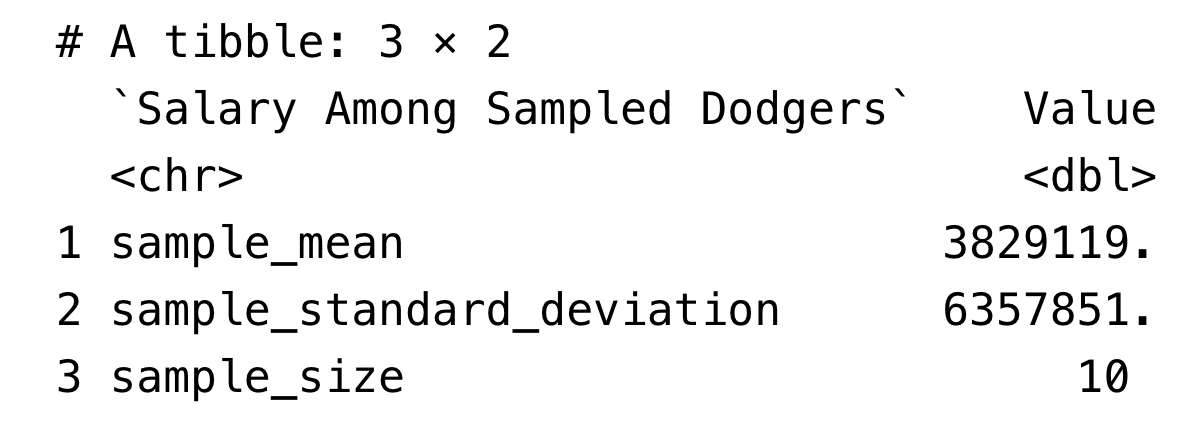
\includegraphics[width = .7\textwidth]{figures/salary_data}

\end{frame}

\section{Classical Inference}

\begin{frame}{Estimator: Sample mean}

$$\hat\mu = \frac{1}{n}\sum_{i}Y_i$$

\end{frame}

\begin{frame}{Variance of the sample mean}

$$
V(\hat\mu) = V\left(\frac{1}{n}\sum_i Y_i\right) = \frac{1}{n^2}\sum_i V(Y_i) = \frac{V(Y)}{n}
$$
Standard error:
$$
\text{SD}(\hat\mu) = \sqrt{\text{V}(\hat\mu)} = \frac{\text{SD}(Y)}{\sqrt{n}}
$$

\end{frame}

\begin{frame}{Asymptotic normality}

$$
\hat\mu \rightarrow \text{Normal}\left(\text{Mean} = \text{E}(Y),\quad \text{SD} = \frac{\text{SD}(Y)}{\sqrt{n}}\right)
$$

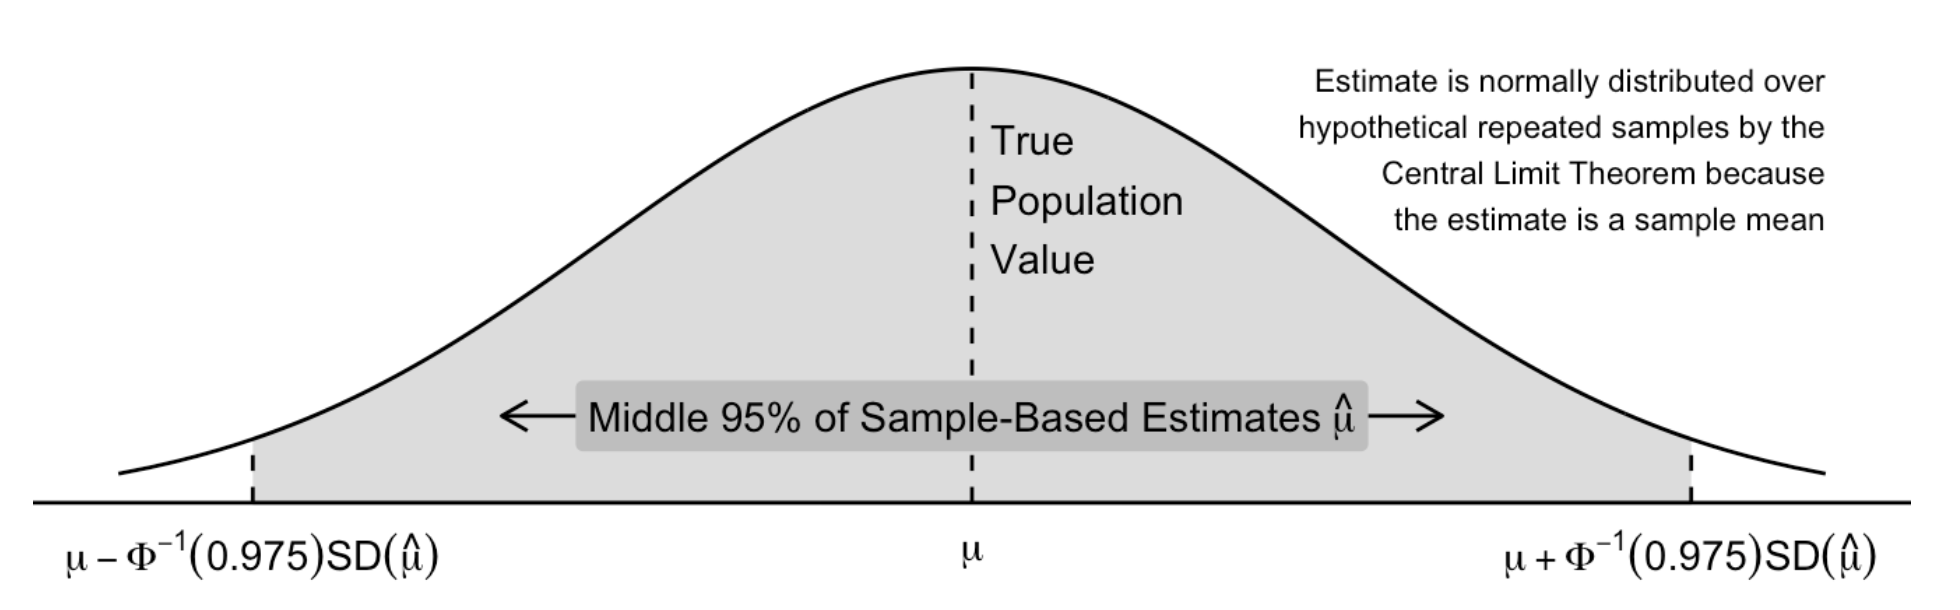
\includegraphics[width = \textwidth]{figures/sampling_distribution}

\end{frame}

\begin{frame}{Asymptotic normality: Even if $Y$ is not Normal}

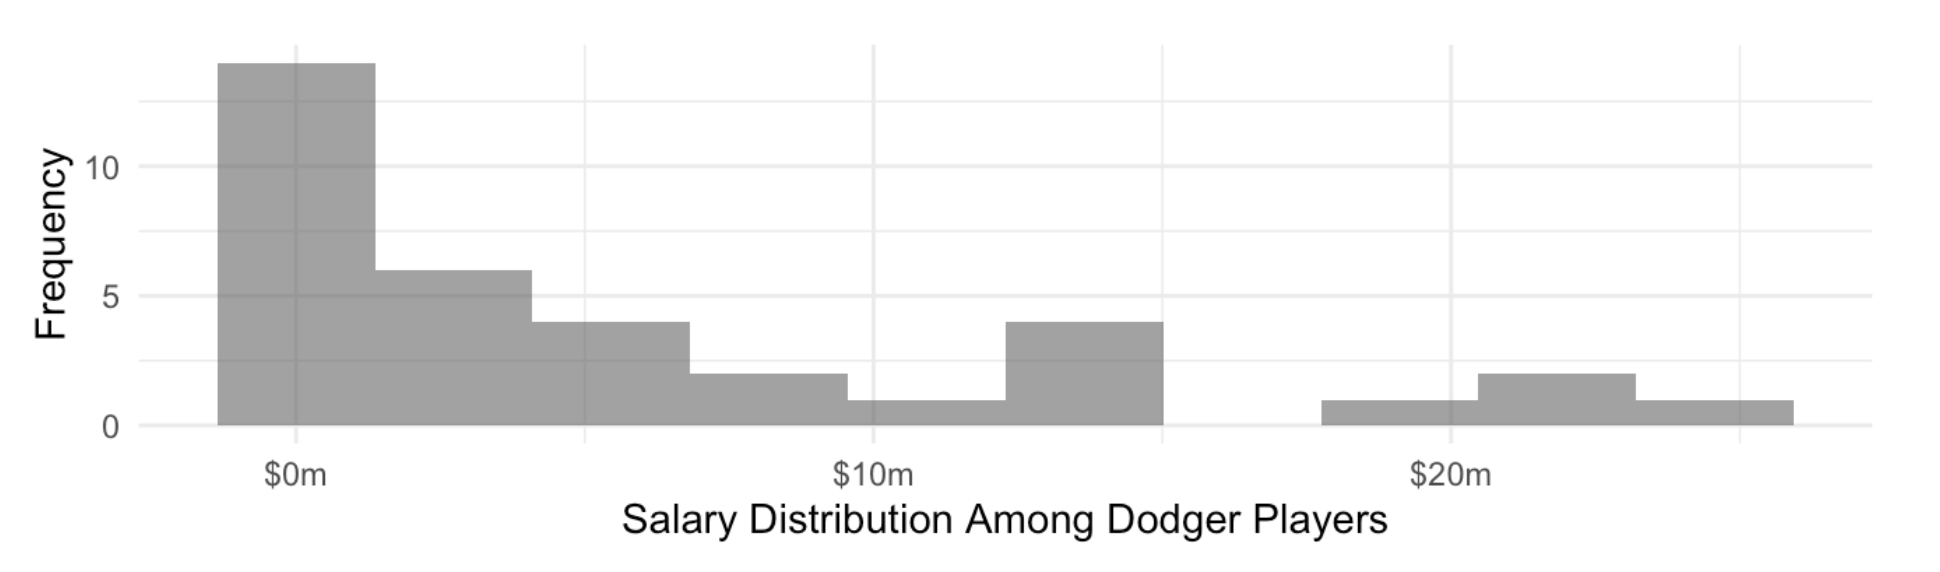
\includegraphics[width = \textwidth]{figures/clt_before} \pause
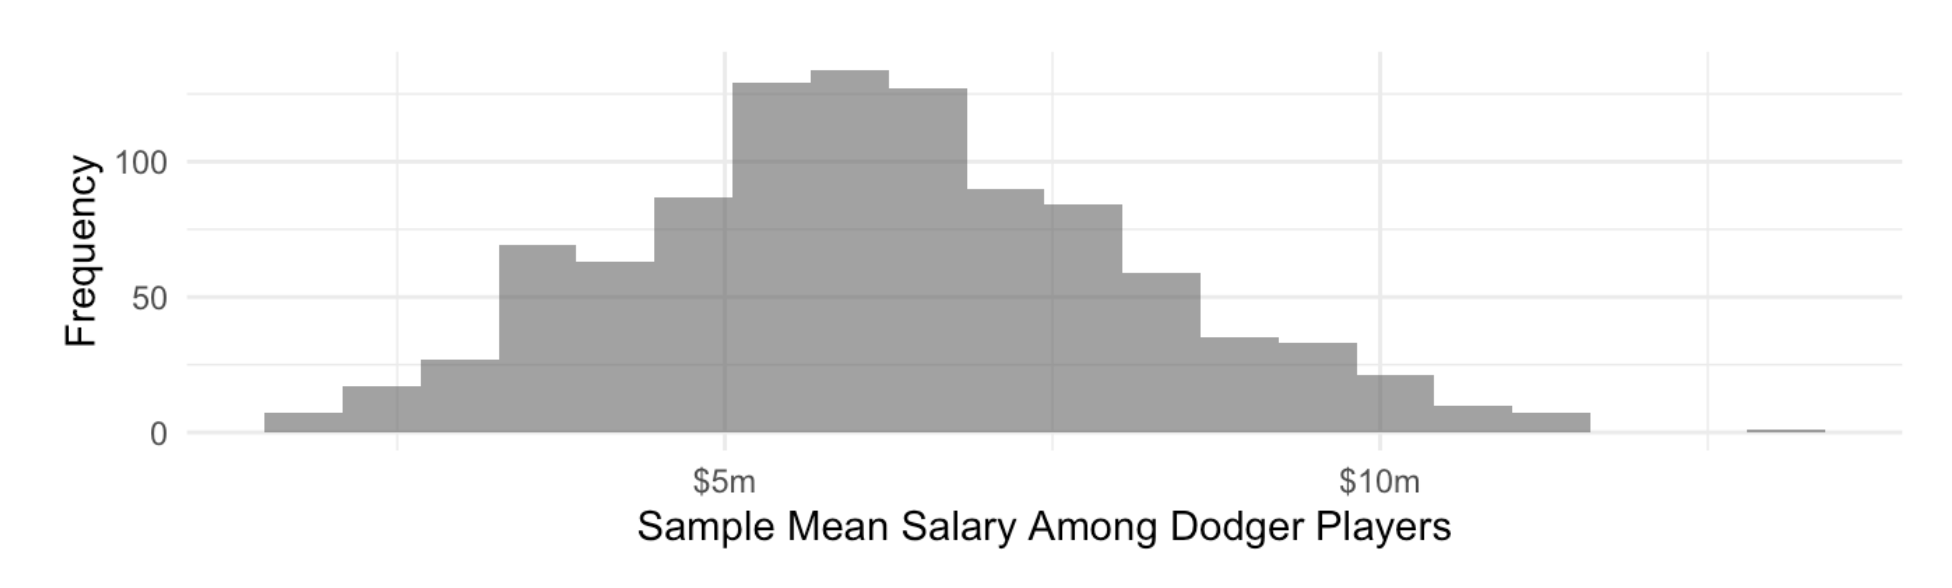
\includegraphics[width = \textwidth]{figures/clt_after}


\end{frame}

\begin{frame}{The plug-in principle}

When you need a population parameter (e.g., $\text{SD}(y)$),\\use the sample-based analog

$$
\widehat{\text{SD}}(\hat\mu) = \frac{\widehat{\text{SD}}(Y)}{\sqrt{n}} = \sqrt{\frac{\frac{1}{n-1}\sum_i (Y_i - \bar{Y})^2}{n}}
$$

\end{frame}

\begin{frame}{Confidence intervals}

What is a 95\% confidence interval for $\mu$? \pause

It is $(\hat\mu_\text{Lower},\hat\mu_\text{Upper})$ such that

$$
\begin{aligned}
\text{P}(\hat\mu_\text{Lower} > \mu) &= .025 \\
\text{P}(\hat\mu_\text{Upper} < \mu) &= .025
\end{aligned}
$$

You may know this formula:

$$
\hat\mu \pm \Phi^{-1}(.975)\widehat{\text{SD}}(\hat\mu)
$$
where $\Phi^{-1}(.975)$ is the value 1.96 that you might look up in the back of a statistics textbook.
\end{frame}

\begin{frame}{Proof of confidence interval formula}
$$
\begin{aligned}
&\text{P}\left(\hat\mu_\text{Lower} > \mu\right)\\ \pause
&=\text{P}\left(\hat\mu - \Phi^{-1}(.975)\widehat{\text{SD}}(\hat\mu) > \mu\right)\\ \pause
&= \text{P}\left(\hat\mu - \mu > \Phi^{-1}(.975)\widehat{\text{SD}}(\hat\mu)\right)\\ \pause
&= \text{P}\left(\frac{\hat\mu - \mu}{\widehat{\text{SD}}(\hat\mu)} > \Phi^{-1}(.975)\right)\\ \pause
&= .025
\end{aligned}
$$

\end{frame}

\begin{frame}

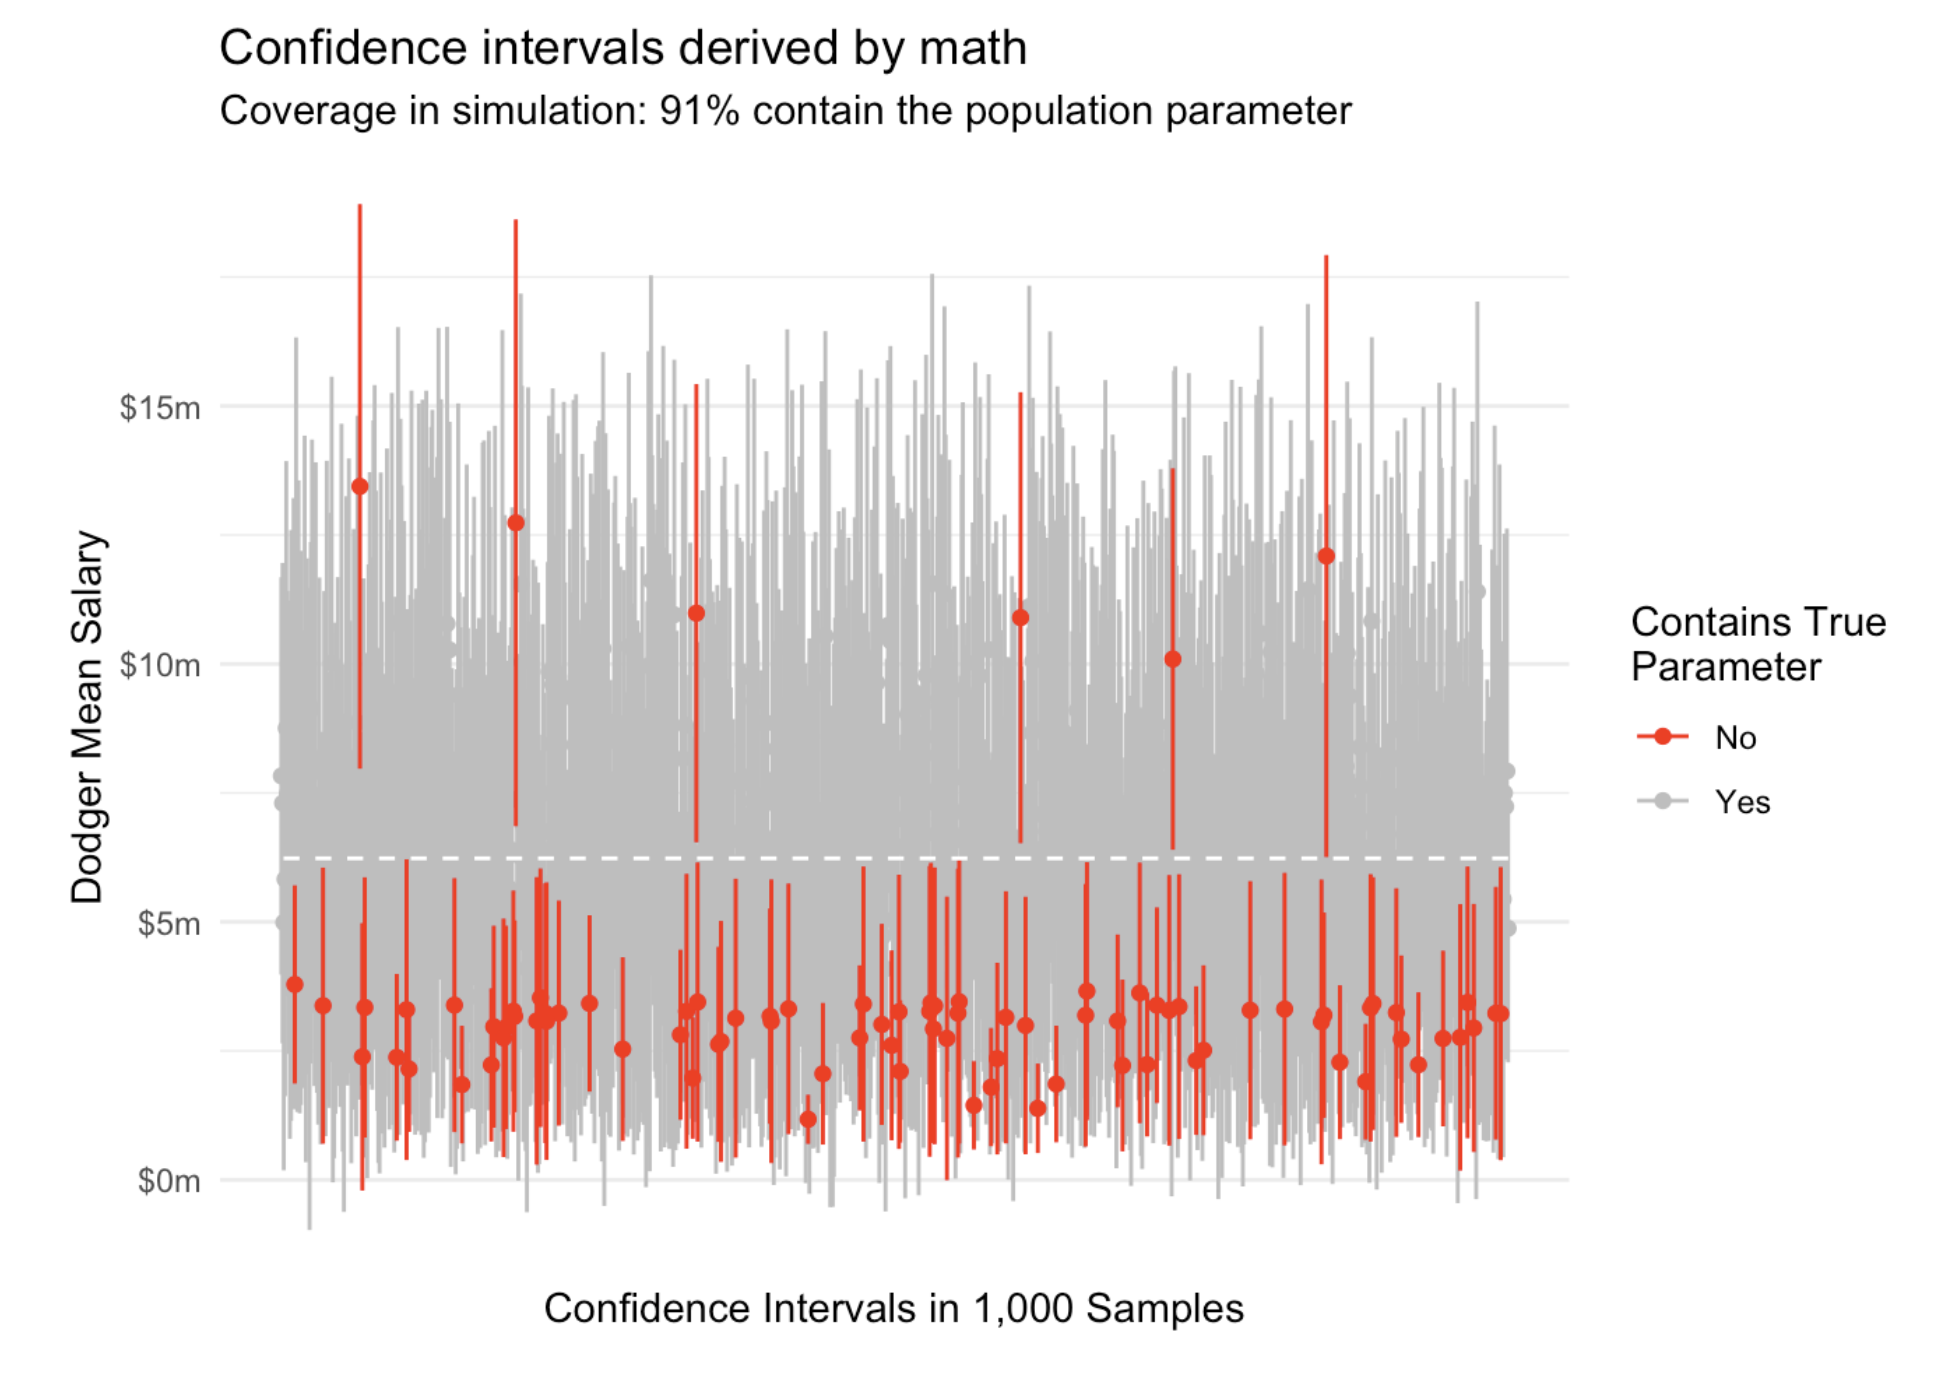
\includegraphics[width = \textwidth]{figures/analytic_cis}
\end{frame}

\begin{frame}

Now suppose you had a complicated data science approach, such as a predicted value $\hat{Y}_{\vec{x}}=\hat{\text{E}}(Y\mid \vec{X} = \vec{x})$ from a LASSO regression. \vskip .2in

How would you place a confidence interval on that predicted value?

\end{frame}

\section{Bootstrap}

\begin{frame}{How our estimate comes to be}

$$F\rightarrow \texttt{data} \rightarrow s(\texttt{data})$$ \pause

\begin{enumerate}
\item The world produces data \pause
\item Our estimator function $s()$ converts data to an estimate
\end{enumerate} \vskip .1in

\begin{center}
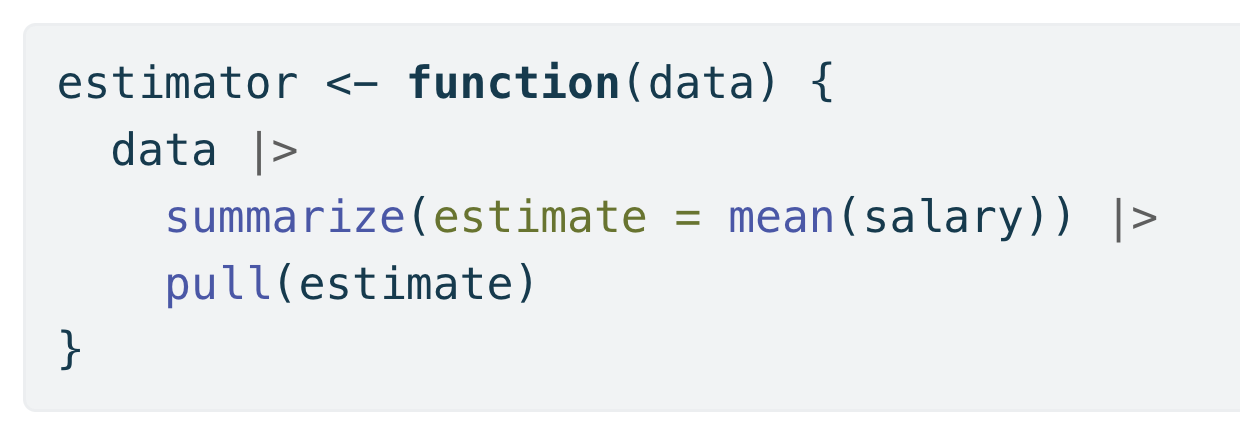
\includegraphics[width = .7\textwidth]{figures/estimator}
\end{center}

\end{frame}

\begin{frame}{The bootstrap idea}

$$F\rightarrow \texttt{data} \rightarrow s(\texttt{data})$$ \pause
$$\hat{F}\rightarrow \texttt{data}^* \rightarrow s(\texttt{data}^*)$$ \pause

\begin{itemize}
\item $F$ is the true distribution of data in the population
\item $\hat{F}$ is a plug-in estimator: our empirical data distribution
\end{itemize}

\end{frame}

\begin{frame}{The bootstrap idea}

\begin{enumerate}
\item Generate $\texttt{data}^*$ by sampling with replacement from $\texttt{data}$
\item Apply the estimator function
\item Repeat (1--2) many times. Get a distribution.
\end{enumerate}

\end{frame}

\begin{frame}{Original sample}
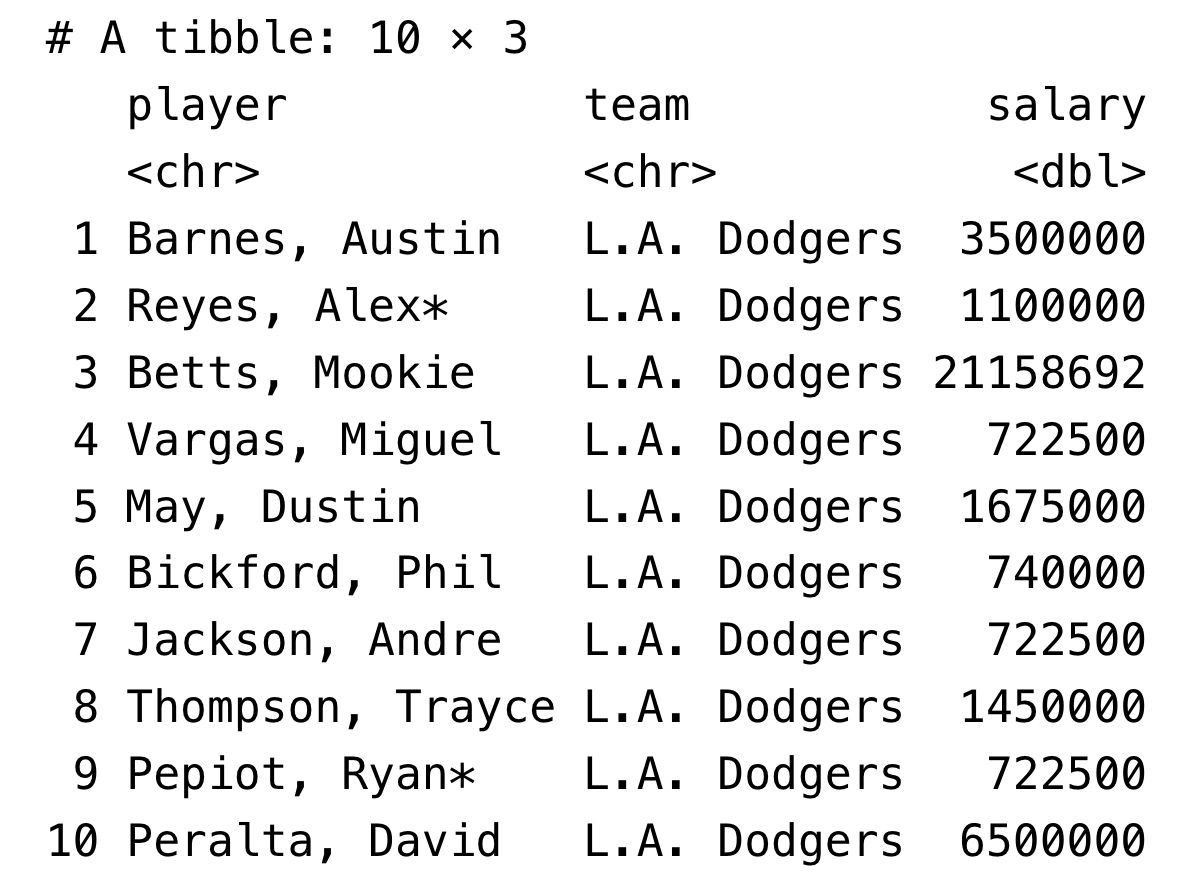
\includegraphics[width = .7\textwidth]{figures/original_sample}
\end{frame}

\begin{frame}{Bootstrap sample}
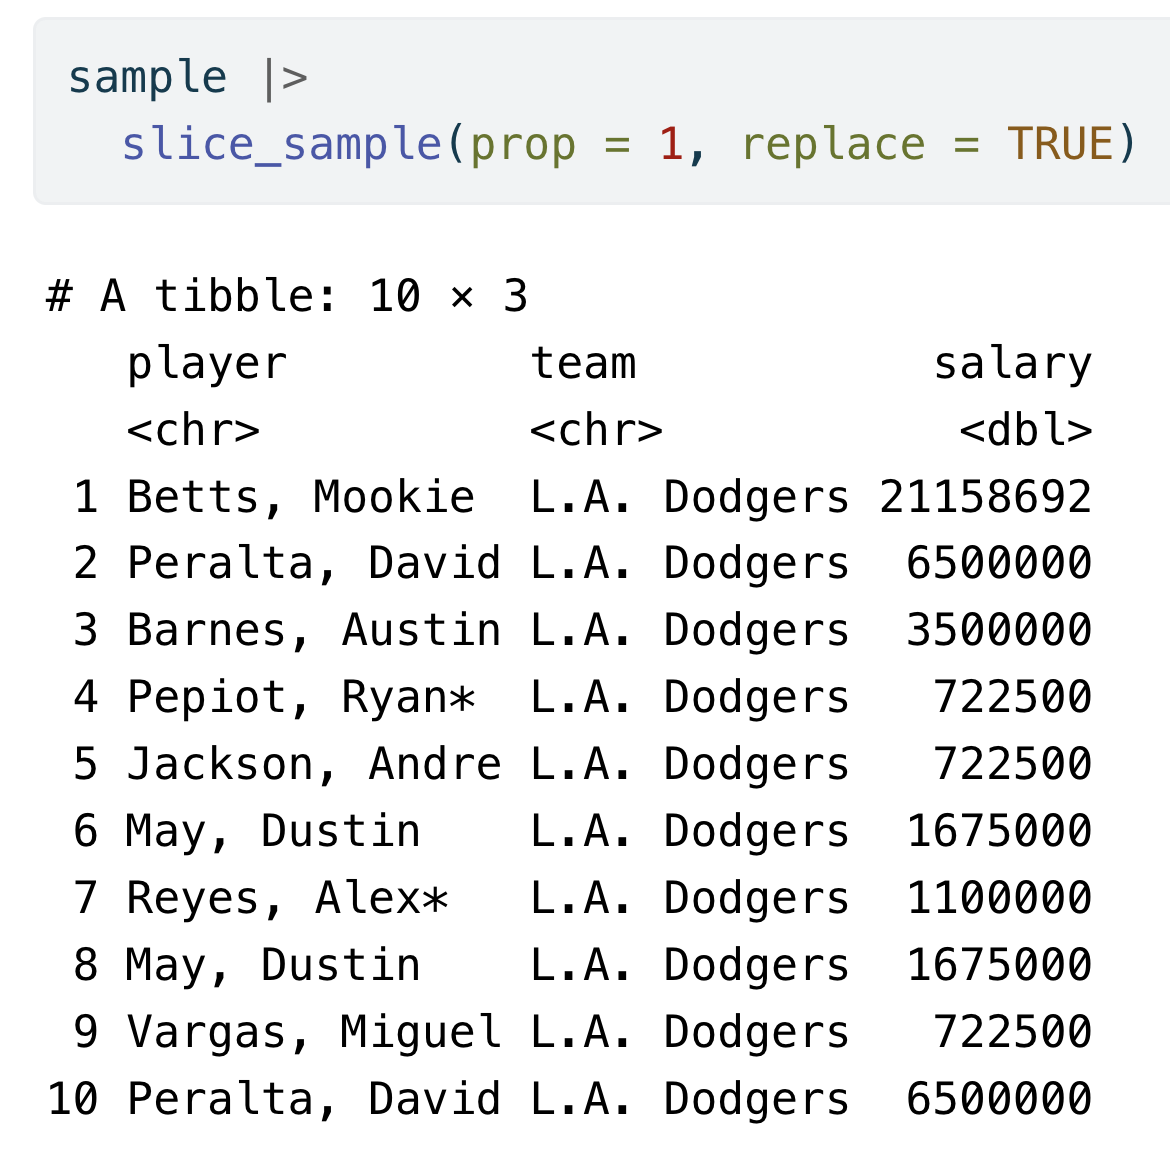
\includegraphics[width = .7\textwidth]{figures/bootstrap_sample}
\end{frame}

\begin{frame}{Bootstrap: Many sample estimates}
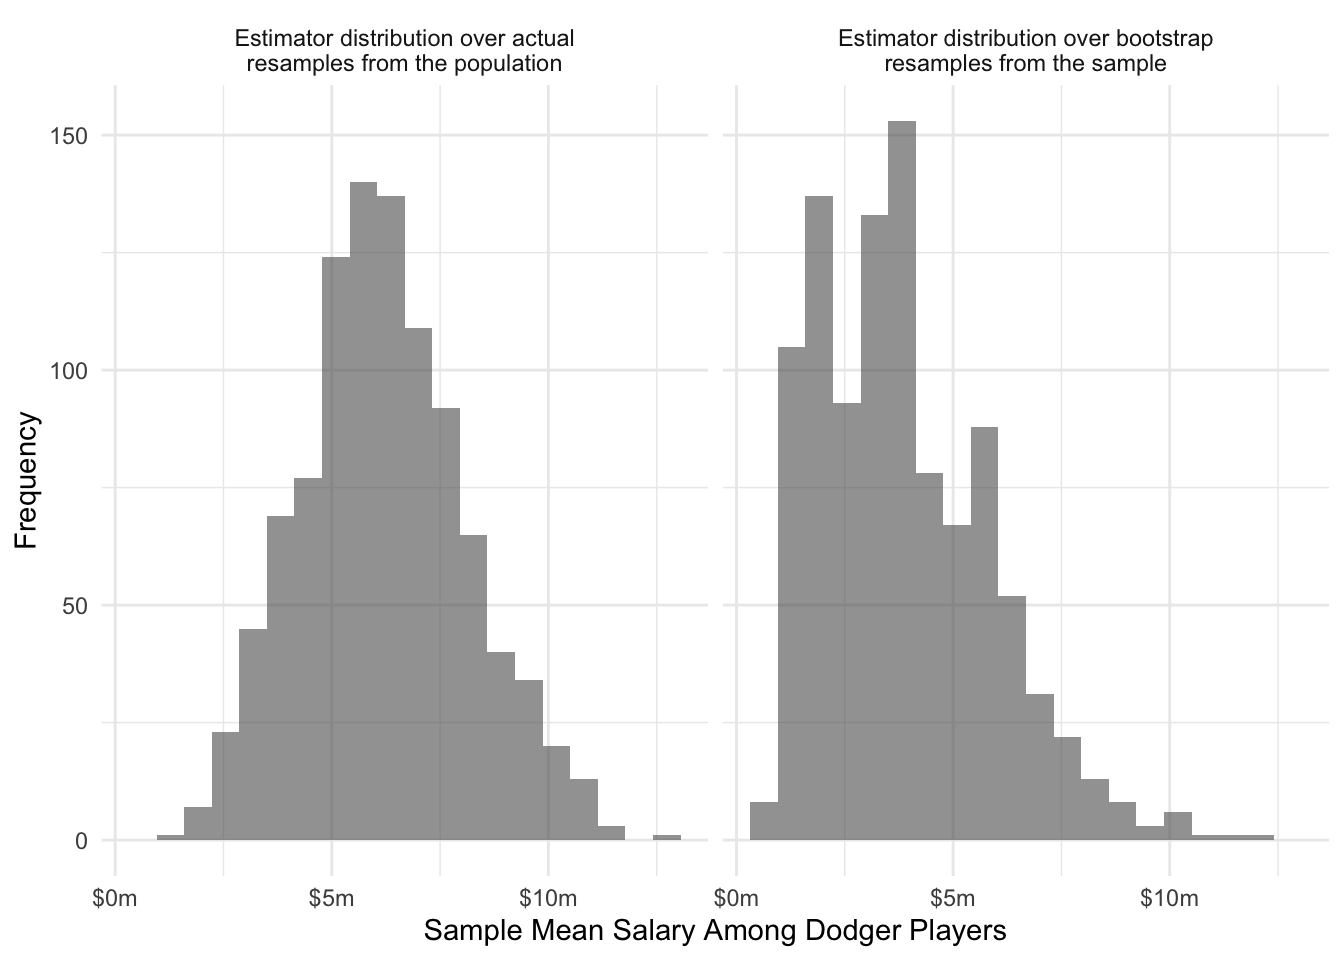
\includegraphics[width = \textwidth]{figures/bs_dist}
\end{frame}

\begin{frame}{Bootstrap standard errors} \pause

\textbf{Goal:} Standard deviation across hypothetical sample estimates \pause \\
\textbf{Estimator:} Standard deviation across bootstrap estimates
$$
\widehat{\text{SD}}(s) = \frac{1}{B-1}\sum_{r=1}^B \bigg(s(\texttt{data}^*_r) - s(\texttt{data}^*_\bullet)\bigg)^2
$$

\end{frame}

\begin{frame}{Bootstrap confidence intervals}

Two (of many) approaches
\begin{itemize}
\item normal approximation
\item percentile method
\end{itemize}

\end{frame}

\begin{frame}{Bootstrap confidence intervals}{Normal approximation}

Point estimate + Bootstrap Standard Error + Normal Approximation \pause \vskip .2in
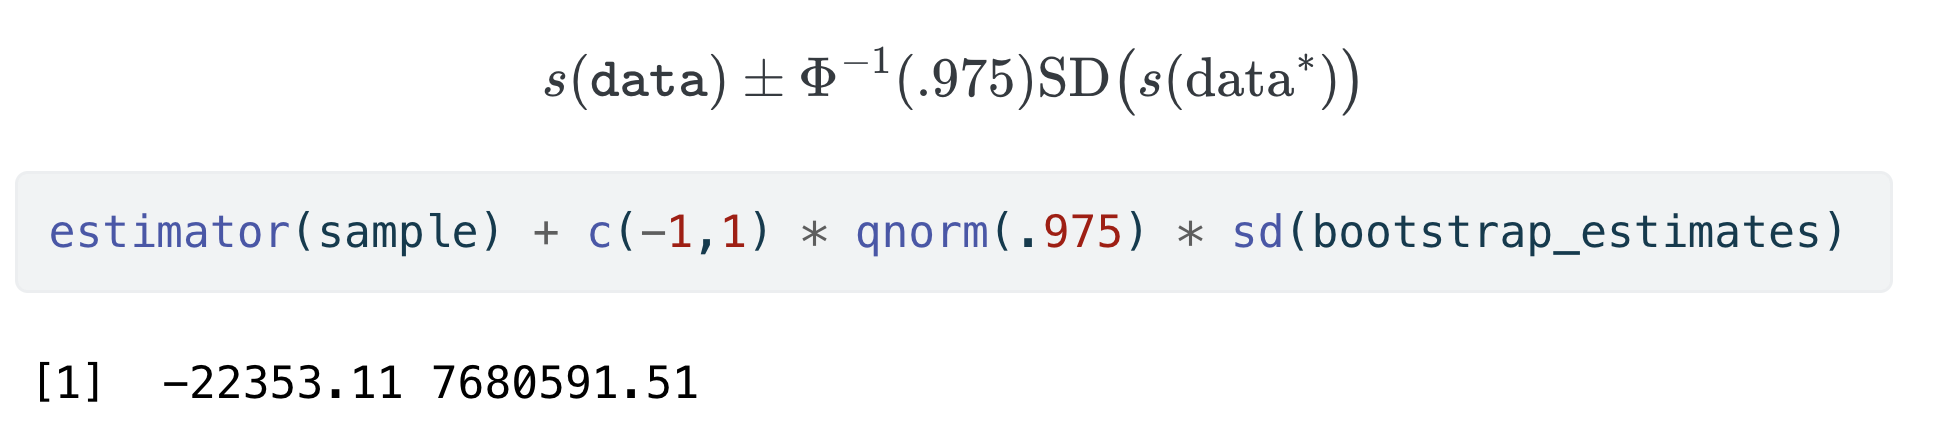
\includegraphics[width = \textwidth]{figures/bs_normal}

\end{frame}

\begin{frame}{Bootstrap confidence intervals}{Percentile method}

Point estimate + Bootstrap Distribution + Percentiles \pause \vskip .2in
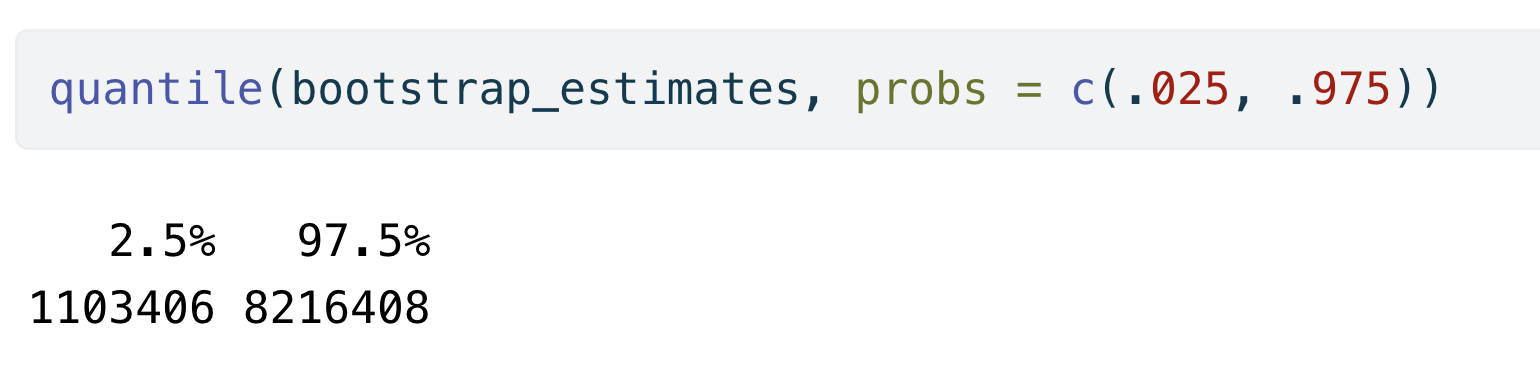
\includegraphics[width = \textwidth]{figures/bs_percentile} \vskip .1in
(requires a larger number of bootstrap samples)

\end{frame}

\section{Discussion}

\begin{frame}{Bootstrap discussion: 1 of 2}

Suppose a researcher carries out the following procedure.

\begin{enumerate}
\item Sample $n$ units from the population
\item Learn an algorithm $\hat{f}:\vec{X}\rightarrow Y$ to minimize squared error
\item Report a prediction $\hat{\text{E}}(Y\mid\vec{X} = \vec{x}) = \hat{f}(\vec{x})$
\end{enumerate}

How would the researcher use the bootstrap to carry out this process? \pause

\begin{enumerate}
\item Draw a bootstrap sample $\texttt{data}^*$ of size $n$
\item Learn the algorithm $\hat{f}^*$ in the bootstrap sample
\item Store the bootstrap estimate $\hat{f}^*(\vec{x})$
\end{enumerate}
Then percentiles or normal approximation! \vskip .1in

Note that a biased estimator may undermine coverage; we will return at the end to this.

\end{frame}

\begin{frame}{Bootstrap discussion: 2 of 2}

In each example, describe the steps the researcher might use to bootstrap this estimate while capturing all sources of uncertainty.

\begin{enumerate}
\item A researcher first truncates the values of a skewed predictor variable $x$ at the 1st and 99th percentile. Then the researcher learns a regression model and reports $\hat\beta$. \pause
\item A researcher first uses cross-validation to select the tuning parameter $\lambda$ for ridge regression. Then, they estimate ridge regression with the chosen $\lambda$ value and make a prediction $\hat{f}(\vec{x})$ at some predictor value $\vec{x}$ of interest. \pause
\item A researcher first learns a prediction function $\hat{f}:\vec{X}\rightarrow Y$ and then sees which subgroup $\vec{x}$ has the highest predicted value $\hat{f}(\vec{x})$, which the researcher reports.
\end{enumerate}

\end{frame}

\section{Complex Samples}

\begin{frame}{Complex samples}
\begin{itemize}
\item stratified
\item clustered
\item beyond
\end{itemize}
\end{frame}

\begin{frame}{Simple random sample}
Sample 150 players at random.\\
(standard bootstrap applies)
\end{frame}

\begin{frame}{Stratified sample}
Sample 10 players on each of 30 teams
\begin{itemize}
\item Why doesn't the simple bootstrap mimic this sampling variability well?
\end{itemize} \pause
\vskip .2in
Solution: Stratified bootstrap
\begin{itemize}
\item Take resamples within groups
\item Preserve distribution across groups
\end{itemize}
\end{frame}

\begin{frame}{Clustered sample}
Sample 10 teams. Record data on all players in sampled teams.
\begin{itemize}
\item Why doesn't the simple bootstrap mimic this sampling variability well?
\end{itemize} \pause
\vskip .2in
Solution: Cluster bootstrap
\begin{itemize}
\item Bootstrap the groups
\end{itemize}
\end{frame}

\begin{frame}{Complex survey sample}

\begin{itemize}
\item Often stratified and clustered, in multiple stages
\item Strata and clusters are often restricted geographic identifiers
\end{itemize}

\end{frame}

\begin{frame}{Complex survey sample: Replicate weights}

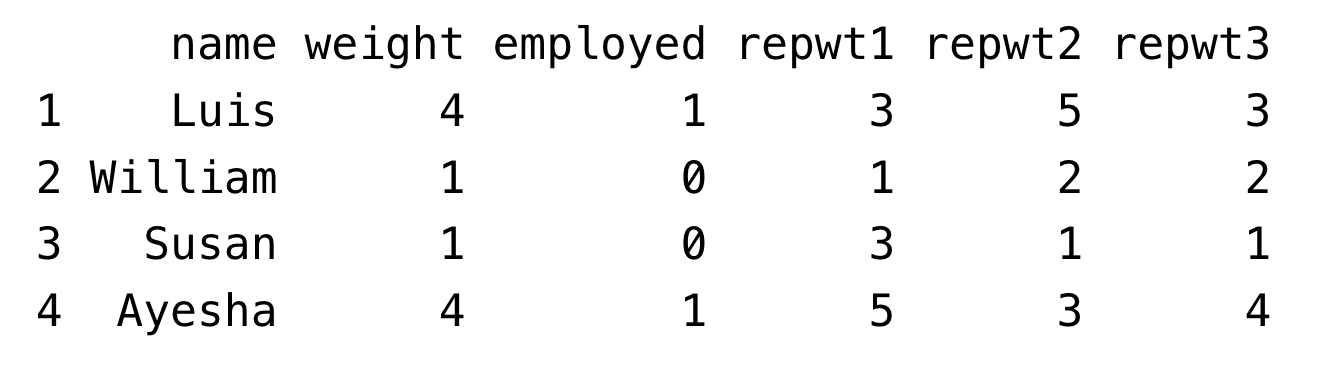
\includegraphics[width = .8\textwidth]{figures/repwt_simple} \vskip .2in
\begin{itemize}
\item Point estimate $\hat\tau$
\item Replicate estimates $\hat\tau^1,\hat\tau^2,\dots$
\end{itemize}

\end{frame}

\begin{frame}{Complex survey sample: Replicate weights}

Re-aggregate as directed by survey documentation.\\
Current Population Survey (example with \href{https://cps.ipums.org/cps/repwt.shtml}{\textcolor{blue}{documentation}}) \pause

$$\text{StandardError}(\hat\tau) = \sqrt{\frac{4}{160}\sum_{r=1}^{160}\left(\hat\tau^*_r - \hat\tau\right)^2}$$

\end{frame}

\section{Words of Warning}

\begin{frame}{Words of Warning}

The bootstrap makes inference easy, but there are catches. \vskip .2in

\begin{itemize}
\item biased estimator
\begin{itemize}
\item<2-> not centered correctly $\rightarrow$ undercoverage
\end{itemize}
\item estimator is something like $\text{max}(\vec{y})$
\begin{itemize}
\item<3-> $\text{max}(\vec{y}^*)$ never above $\text{max}(\vec{y})$
\item<4-> depends heavily on a particular point
\end{itemize}
\end{itemize}

\end{frame}

\goalsframe

\end{document}
